% Canonical-coloring existence from the uncolored transition matrix.
\section{Existence of canonical colorings from the transition matrix}
\label{cc-exist:section}
We use the convention of the Delta notes: a CC coloring has disjoint red
and blue ranges. Its subsequent canonical recoloring is called an RCC.
In this road-coloring discussion we impose the road-coloring assumptions: $\mathcal A$ is the adjacency
matrix of a finite simple two-out directed graph, and
$A=\mathcal A/2=(R+B)/2$ is stochastic, traceless, irreducible and
aperiodic. For source $x$, its two destinations $i=xR$ and $j=xB$ satisfy
$i\ne j$, $i\ne x$, and $j\ne x$. All nullspaces below are right
nullspaces over the real numbers. The criterion remains valid under weaker
hypotheses, but no such weakening changes the setting of this discussion.

Construct the undirected target-pair graph $H_A$ by joining the two
destinations in each row of $A$. The two destinations are distinct, so $H_A$ has no loops.
Different sources may yield the same auxiliary edge; retain its multiplicity
or suppress duplicates, since neither changes bipartiteness.
Let $c$ be the number of its connected components, and let $b$ be the
number of components that are bipartite, with bipartiteness determined by the absence of odd cycles.
Its component partition is the graph-intrinsic canonical partition, not
in general a kernel partition or a red/blue target partition.

\begin{theorem}\label{cc-exist:equivalences}
The following conditions are equivalent:
\begin{enumerate}
\item The graph admits a CC coloring.
\item There exists $s\in\{+1,-1\}^n$ with $As=0$.
\item $H_A$ is bipartite.
\item $\dim\ker A=c$.
\item For any coloring $A=(R+B)/2$ and $\Delta=(R-B)/2$,
$\dim\ker A=\dim\ker\Delta$.
\end{enumerate}
In fact $\dim\ker A=b$ and $\dim\ker\Delta=c$.
\end{theorem}
\begin{proof}
For a row with destinations $i,j$, the equation $As=0$ is
$s_i+s_j=0$. A sign solution is therefore precisely a bipartition of $H_A$.
Color its positive-target edge red and its negative-target edge blue.
The resulting ranges are disjoint and cover all vertices, since irreducibility
ensures that every vertex occurs as a destination. Conversely a CC coloring
assigns signs to its two target sets and supplies a sign solution.

For an arbitrary real column $x$, the equation $Ax=0$ requires
$x_i=-x_j$ across every edge of $H_A$. A bipartite component contributes
one free parameter; an odd cycle, including a loop, forces every value
on its component to vanish. Thus $\dim\ker A=b$.
The equation $\Delta x=0$ instead requires $x_i=x_j$ across every edge,
independently of the coloring. Its solutions are exactly the columns
constant on components, so $\dim\ker\Delta=c$.
\end{proof}

\subsection{Constructing and counting the CC colorings}
Given a sign solution, put $g=\operatorname{diag}(s)$. Then
\[
 R_{\mathrm{CC}}=A(I+g),\qquad B_{\mathrm{CC}}=A(I-g),
 \qquad \Delta_{\mathrm{CC}}=Ag,
 \qquad A=\Delta_{\mathrm{CC}}g.
\]
Each row of these matrices selects one of the original outgoing edges.
If $H_A$ is bipartite, its $c$ components can be oriented independently,
giving exactly $2^c$ labeled CC colorings or $2^{c-1}$ up to global
red/blue interchange. Every target is incident to an auxiliary edge,
so distinct sign choices give distinct colorings.
Changing the signs on a target component induces row swaps at its
predecessor source vertices, which need not be the vertices of the
component itself. This distinction matters when implementing recolorings.

A breadth-first or depth-first bipartiteness test either constructs the
signs or returns an odd-cycle obstruction. Thus existence is decidable
without enumerating all row recolorings.


\subsection{A four-state illustration of the target-pair test}
\label{cc-exist:four-state-graph}
Consider $R=[4312]$ and $B=[3443]$. The two targets at each source give
\[
 \{4,3\},\quad\{3,4\},\quad\{1,4\},\quad\{2,3\}.
\]
Ignoring the repeated edge, the auxiliary graph is the path $1-4-3-2$.
It is bipartite, with sides $\{1,3\}$ and $\{2,4\}$. These sides are
\emph{target types}, not kernel blocks. The auxiliary graph is connected,
so its component partition has just one block.

Choose $\{1,3\}$ as the red target side. At each source, color the edge
ending on that side red and the other edge blue. This swaps the outgoing
colors at sources 1 and 4, producing
\[
 R_{\mathrm{CC}}=[3313],\qquad B_{\mathrm{CC}}=[4442].
\]
Their ranges are disjoint: $\operatorname{Im}R_{\mathrm{CC}}=\{1,3\}$
and $\operatorname{Im}B_{\mathrm{CC}}=\{2,4\}$. The original coloring
is not CC, since its red and blue ranges overlap. Thus bipartiteness tests
\emph{existence of a CC recoloring}, not whether the supplied coloring is
already CC. Swapping the two target types gives the only other labeled CC
choice. The swaps here construct a CC coloring; they are not the subsequent
CC-to-RCC canonical recoloring operation.

\begin{figure}[tbp]
\centering
\begin{minipage}[t]{0.48\textwidth}
\centering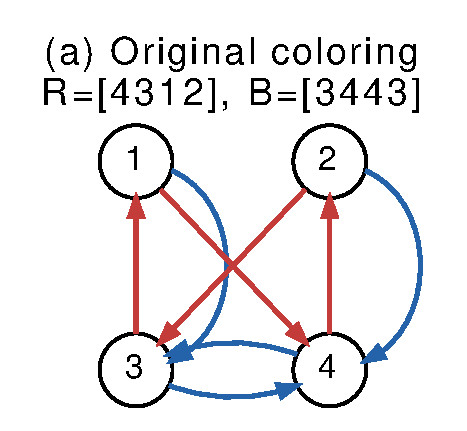
\includegraphics[width=\linewidth]{cc-original.eps}
\end{minipage}\hfill
\begin{minipage}[t]{0.48\textwidth}
\centering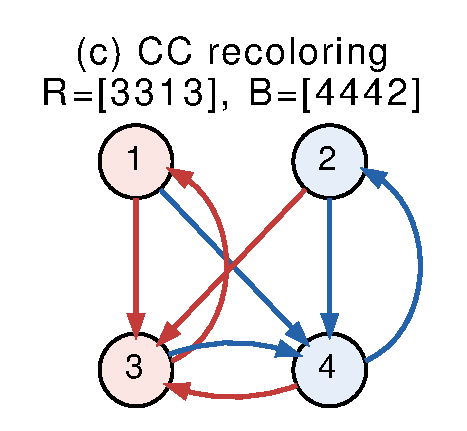
\includegraphics[width=\linewidth]{cc-cc.eps}
\end{minipage}

\medskip
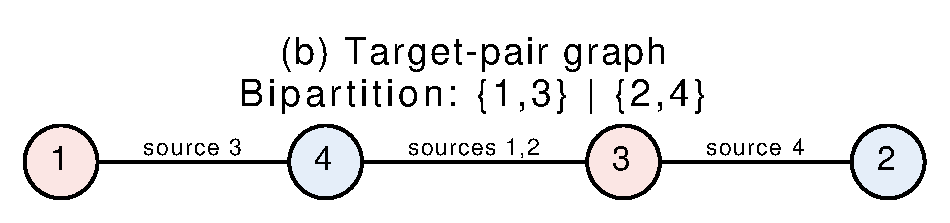
\includegraphics[width=0.92\textwidth]{cc-target.eps}
\caption{The four-state CC test. Top: (a) the original coloring and
(c) its CC recoloring, with red $R$-arrows and blue $B$-arrows.
Bottom: (b) the undirected target-pair graph; its edge $\{3,4\}$ comes
from both sources 1 and 2. Tinted vertices indicate the chosen red and
blue target types. The directed graph is unchanged; only the outgoing
colors at sources 1 and 4 are interchanged.}
\label{fig:cc-four-state-target-pair}
\end{figure}

\subsection{A test involving only matrix operations on $A$}
Define
\[
 L_A=\operatorname{diag}(A^{\mathsf T}\mathbf1)-A^{\mathsf T}A.
\]
\begin{proposition}\label{cc-exist:matrix-test}
For every coloring,
\[
 L_A=\Delta^{\mathsf T}\Delta.
\]
Consequently $L_A$ is positive semidefinite, $\dim\ker L_A=c$, and
\[
 \text{CC exists}\quad\Longleftrightarrow\quad
 \operatorname{nullity}A=\operatorname{nullity}L_A.
\]
\end{proposition}
\begin{proof}
Let $u=e_i$, $v=e_j$ be the two destination columns for one row.
That row contributes
\[
 \tfrac12(uu^{\mathsf T}+vv^{\mathsf T})
 -\tfrac14(u+v)(u+v)^{\mathsf T}
 =\tfrac14(u-v)(u-v)^{\mathsf T}
\]
to $L_A$. This is also its contribution to $\Delta^{\mathsf T}\Delta$,
regardless of which edge is red. The identity holds when $i=j$ as well.
Summing proves it, and the nullspace assertions follow from
$\ker(\Delta^{\mathsf T}\Delta)=\ker\Delta$ and
Theorem~\ref{cc-exist:equivalences}.
\end{proof}
The identity uses the equally weighted two-out hypothesis. It should not
be applied unchanged to an arbitrary stochastic matrix.

\subsection{Singularity is necessary but not sufficient}
An invertible $A$ rules out CC colorings. A singular $A$ need not admit one:
some components of $H_A$ may be bipartite while others are not.
For example, take
\[
 R=[24111],\qquad B=[35233].
\]
The directed graph is irreducible and aperiodic, while $H_A$ consists of
a triangle on $\{1,2,3\}$ and an edge on $\{4,5\}$. Therefore
\[
 \ker A=\operatorname{span}\{(0,0,0,1,-1)^{\mathsf T}\},
 \qquad \dim\ker\Delta=2.
\]
The transition matrix is singular, but no sign solution exists and there
is no CC coloring. If $H_A$ is connected, on the other hand, singularity
of $A$ is sufficient as well as necessary.

\subsection{Existence versus kernel rank}
These tests decide existence and construct all CC colorings; they do not
force synchronization. Our nine-state graph has two CC choices up to
color interchange, of kernel ranks three and one. Their associated RCCs
have ranks six and two. The six-state CC example $[312344],[666565]$
has a unique CC choice up to interchange; its RCC has partition
$(1234\mid56)$ and rank two.
